\setcounter{page}{1}

\def\theTopic{Intro \& Syllabus }
\def\dayNum{1}


\begin{center}
\vspace*{.1in}
{\bf {\large Stat 216 Syllabus Spring 2016}}\\
\end{center}
\vspace{-.1in}

\begin{center}
  {\bf People}
\end{center}
\begin{itemize}
\item Your Instructor: (Write contact info here) \vspace{5.5cm}
\item Student Success Coordinator:  Jade Schmidt\\
     email: roskam@math.montana.edu\hfill Office: Wilson 2-260 \hfill
     406-994-5357
   \item Course Supervisor: Dr. Robison-Cox\\
     email: jimrc@montana.edu \hfill  Office: Wilson 2-241 \hfill
     406-994-5340
\end{itemize}


\begin{center}
  {\bf Course Materials}
\end{center}
  You need to buy the Stat 216  Course Pack  the MSU
  Bookstore.  It will not work to use an old one from a friend.

  We will  use several online web applications,  so you need
  access to a computer.  You will work as a group of three and one of
  your group needs to bring a computer for each class meeting.\\
 
  We recommend the free online textbook {\it Intro Stat with Randomization and
    Simulation} at \url{https://www.openintro.org/stat/textbook.php}
   for further explanations, but note that they do follow a different
   order of topics than these materials.\\
  Other materials, such as readings and D2Boxes (our word for
  very important homeworks) will be downloaded from D2L, so be
  sure you can log in to the MSU D2L (Brightspace) system:\\
   \url{https://ecat.montana.edu/}.  If you have problems, view the
   help on that page.

  {\bf Recommendation:}  In D2L you can click on your name, go to your
    account settings,  select  the ``Email'' tab, and set {\bf
      Forwarding Options} to send D2L mail to an account which you
    check more regularly.  We strongly recommend that you do this.  We
    might need to send out updates, and forwarding means you will not
    have to login in to D2L to get them.
\newpage

   \begin{center}
     {\bf Learning Outcomes for STAT 216 }
   \end{center}
   \begin{itemize}
   \item Understand how to describe the characteristics of a distribution.
   \item Understand how data can be collected, and how data collection
     dictates the choice of statistical method and appropriate
     statistical inference.
   \item Interpret and communicate the outcomes of estimation and
     hypothesis tests in the context of a problem. We will cover tests
     and estimation in the contexts of: one proportion, one mean, two
     proportions, two means, and a regression slope.   
   \item Understand when we might make causal inference from a
     sample to a population.
   \item Understand how selection of a sample influences the
     group to which we might make inference.
   \end{itemize}
   
    

{\bf CORE 2.0}:  This course fulfills the Quantitative Reasoning (Q)
CORE 2.0 requirement because learning statistics allows us to
disentangle what's really happening in nature from ``noise'' inherent in
data collection. It allows us to evaluate claims from advertisements
and results of polls and builds critical thinking skills which form
the basis of statistical inference.   

{\bf Comments and concerns}: We are always looking for ways to improve
this class and we want students to be successful.  The first step is
to discuss your comments or concerns with your instructor.  If they
are not resolved, contact the Student Success Coordinator, Jade
Schmidt. 

 
{\bf Course Description }
 
Stat 216 is designed to engage students using a 
simulation approach to inference using web apps. Use of  small group
discussion activities and daily assignments have been shown by the
research to be effective. Upon completion of this
course, you should have an understanding of the foundational concepts
of data collection and of inference and you will appreciate the
fundamental role that statistics plays in all disciplines.  In
addition, statistical summaries and arguments are a part of everyday
life, and a basic understanding of statistical thinking is critical
when it comes to helping you become an informed consumer of the
numerical information they encounter on a daily basis.   You will be
exposed to numerous examples of real-world applications of statistics
that are designed to help you develop a conceptual understanding of
statistics.     
 
Note: this course will be a lot of work, and attendance every day is
really important for your success. You will need to prepare for class
every day and to turn in assignments twice per week.

Please think seriously about this as you decide if this course is the
right fit for you.    

\newpage
 
{\bf Prerequisites }
 
You should have completed  a 100-level math course (or equivalent) with
a grade of C- or better (Alternatives: a good score on Math portion
of SAT or ACT, or a 3.5 on the MPLEX exam).   
 You should have familiarity with computers and technology (e.g.,
Internet browsing, word processing, opening/saving files, converting
files to PDF format, sending and receiving e-mail, etc.). See the
Technology section of the syllabus for more details.  
 


{\bf Technology} \vspace{-.3in}
\begin{itemize}
\item {\bf Web Applets}  We will be utilizing web applets 
 at \url{http://shiny.math.montana.edu/jimrc/IntroStatShinyApps/}
  These run in a web browser, but
  may have trouble with older versions of the Microsoft IE browser.
\item {\bf Technology Policy}:  This course utilizes technology
  extensively.  You will need at least one laptop within your group each
  day.
\item {\bf Appropriate Use}: We need to use web apps, but it is NOT OK
  to use other websites during class. {\bf You may not I-chat or text
    with friends or to use web sites other than those we direct you to
    during class.} Our class time is really limited. We need to use it
  for group work and for instructors to give intros, wrapups, and
  reviews.  Students who use technology inappropriately will lose
  attendance or RAT points for the day, and will have to  leave the
  room if they cannot stop such behavior.
\item {\bf Turn OFF your cell phone and put it away}.
\end{itemize}

{\bf Math Learning Center} in 1-112 Wilson Hall is a very important
resource providing  help on Stat 216 topics.
 It is open every day, into the evenings on MTWR, and closes early on
 Friday. 


{\bf Assessment}\\
Your grade in this course will be based on the following: 
\begin{itemize}
\item  {\bf D2Boxes: 15\%}  These assignments  will help you learn
  the course material and software through 
  reflection and practice and are essential preparation for the exam. 

  Format: Your instructors will tell you if you submit these as
  electronic files uploaded to a D2L Dropbox or as hard copies. If electronic,
  it needs to be in a format we can read.  Adobe pdf is our standard.
  Submissions we can't read will not count.

\item {\bf D2L Quizzes:  10\%} These are similar to the D2Box
  assignments, but are graded automatically (mostly) on D2L.

\item {\bf Common Hour Exam I:  20\%}  Taken individually, not
  in groups. You may bring a one handwritten sheet of notes.
\item {\bf Common Hour Exam II:  20\%} Taken individually, not
  in groups. You may bring a one handwritten sheet of notes.
\item {\bf Final Exam:  25\%}.  This exam will be cumulative in
  content. Again, you will be allowed to bring in one page of
  handwritten notes for the final exam.   
 
\item {\bf Attendance/Participation/Preparation:  10\%} . Class
  participation is an important part of learning, especially in
  courses like this one that involve group cooperation.    

  {\it Participation/Attendance}: Students can miss class/arrive
  late/leave early once (1 day) before they will be penalized for
  non-participation due to an absence.  For each day missed
  thereafter, the students’ overall grade will be reduced 1\% (up to
  5\%).   In addition to attending, it's critically important that
  each student participates in class. Lack of participation can result
  in the same penalty as absence.

  {\it Preparation}: The in-class activities and out-of-class assigned
  readings are the primary source of  information for this course.
  Take them seriously, work through them with care, and they will be
  very valuable on exams.  As a way to provide further emphasis to the
  activities and readings, most classes will begin with a Readiness
  Assessment Test (RAT) with questions covering the previous class's
  activity and readings required for the class.   
\end{itemize}

{\it Late or Missed Work}:  If you cannot be in class, it is your 
responsibility to notify the instructor and your group members with as
much advance warning as possible. In general, make-up exams or late
homework assignments will not be allowed. Case-by-case exceptions may
be granted in only extreme cases at the discretion of the
instructor (daily work) or Student Success coordinator (exams). You
must provide documentation explaining your absence for 
the instructor to determine whether an exception should be granted. If
you fail to provide documentation as requested then you will not be
able to make-up missed work at all.   
 
  Letter grades will be assigned using a 10 point scale.
  As an approximation (which will be fine tuned at the end of the semester)
  94 - 100 = A,  90 to 93 = A-, 87 to 89 = B+, etc.
 
{\bf Planning Ahead:}  In our experience, it takes 6 to 9 hours per
week outside of class to achieve a good grade in Stat 216.  By ``good'' we
mean at least a C because a grade of C- or below does not
count toward fulfilling degree requirements.  Many of you set your
goals higher than just getting a C, and we fully support that.  You
need roughly nine hours per week to  review past activities, read
feedback on previous assignments, complete current assignments, and
prepare for the next day's class. 


The administrators in the departmental office are  busy
people. They cannot accept assignments and cannot provide information
about grades (you should check for yourself on D2L).


\begin{center}
{\large\bf University Policies and Procedures }  
\end{center}

{\bf Behavioral Expectations }\\
Montana State University expects all students to conduct themselves as
honest, responsible and law-abiding members of the academic community
and to respect the rights of other students, members of the faculty
and staff and the public to use, enjoy and participate in the
University programs and facilities. For additional information
reference see MSU's Student Conduct Code at: 
\url{http://www2.montana.edu/policy/student_conduct/cg600.html} .
Behavioral expectations and student rights are further discussed at:
\url{http://www.montana.edu/wwwds/studentrights.html} . 
 

 {\bf Collaboration }\\
Discussing assignments with others (in your group for example) is a
good way to learn.  Giving others answers is not doing them a favor,
because then they aren't learning the material.  Copying from others
is cheating, and will not be tolerated.  
University policy states that, unless otherwise specified, students
may not collaborate on graded material. Any exceptions to this policy
will be stated explicitly for individual assignments. If you have any
questions about the limits of collaboration, you are expected to ask
for clarification. 


 {\bf Plagiarism  }\\
Paraphrasing or quoting anothers work without citing the source is a
form of academic misconduct. Even inadvertent or unintentional misuse
or appropriation of anothers work (such as relying heavily on source
material that is not expressly acknowledged) is considered
plagiarism. If you have any questions about using and citing sources,
you are expected to ask for clarification. 

 {\bf Academic Misconduct  }\\
Section 420 of the Student Conduct Code describes academic misconduct
as including but not limited to plagiarism, cheating, multiple
submissions, or facilitating others’ misconduct. Possible sanctions
for academic misconduct range from an oral reprimand to expulsion from
the university. 

Section 430 of the Student Code allows the instructor to impose the
following sanctions for academic misconduct: oral reprimand; written
reprimand; an assignment to repeat the work or an alternate
assignment; a lower or failing grade on the particular assignment or
test; or a lower grade or failing grade in the course.  

 {\bf Academic Expectations  }\\
Section 310.00 in the MSU Conduct Guidelines states that students
must:\vspace{-.15in}
\begin{list}{}{}
\item[A.] be prompt and regular in attending classes;
\item[B.] be well prepared for classes; 
\item[C.] submit required assignments in a timely manner;
\item[D.] take exams when scheduled;
\item[E.] act in a respectful manner toward other students and the
  instructor and in a way that does not detract from the learning
  experience; and 
\item[F.] make and keep appointments when necessary to meet with the
  instructor.  
In addition to the above items, students are expected to meet any
additional course and behavioral standards as defined by the
instructor. 
\end{list}

  {\bf Withdrawal Deadlines  }\\
 January 27, 2016 is the last day to withdraw without a ``W'' grade.
 University policy is explicit that the adviser and instructor must
 approve requests to withdraw from a course with a grade of ``W''. 
 Students who stop attending and stop doing the work are not
 automatically dropped.  Taking a ``W'' does not hurt your GPA but it
 is a sign that you are not making progress toward your degree, and
 could affect your financial aide or student loans. 

% \newpage

 {\bf Group Expectations }\\
 We have all been in groups which did not function well.  Hopefully,
 we've also all had good experiences with working in groups.  Our use
 of groups in this course is based on educational research which
 provides strong evidence that working in groups is effective and helps
 us learn.  By expressing your opinions and catching each others
 mistakes, you will learn to communicate statistical concepts.  These
 are partly ``common sense''
 ideas (for instance, gathering more data provides a better foundation
 for decision making),  but they are often  phrased in
 odd ways. We find it really helps to talk about them  with
 others. 

% Your instructors will assign groups and will lead you through an
% activity to get to know each other. We'd like your honest opinions
% about what you need from your group and what you fear about working
% with a group.


 \def\theTopic{Fraud Detection}
\newpage


\begin{center}
{\bf  Detecting Fraud }\\
\end{center}
\vspace{-.2in}

Randomness is a key concept in statistics, but how good are we are
detecting randomness, or better yet, at detecting fraud?  We will
investigate this idea today. 

\textbf{With your group:}
\begin{enumerate}
  \item Write down a sequence of 45 coin flips (so 45 heads and tails)
    that you (as a group) think is random. 
\begin{students}
  \vspace{1cm}
\end{students}    
\begin{key}
   {\it Answers will vary. (AWV)}
\end{key}

  \item Now flip your coin 45 times and write down the result of each
    flip. \vspace{.5in} 
\begin{students}
  \vspace{1cm}
\end{students}    
\begin{key}
   {\it Answers will vary. AWV.}
\end{key}

  \item Flip one more coin.  If you get heads, label the second
    sequence of actual flips as sequence ``A'', the ``made up'' flips
    as sequence ``B''.  If you get tails, label them oppositely.
    Don't let other groups see which is which.

    Write both sequences on the board in shorthand with the number
    of consecutive heads or tails, so the sequence {\sf HHHTTHHT} will
    be recorded as:\\
    {\sf 3H\\2T\\2H\\T}

  \item As the other groups write their sequences on the board, 
    guess whether A or B was really the coin flip sequence.  Mark
    your guesses for the sequence from the coin in the table below.
    Each person should guess individually and not as a group!  
    When you come to your own group, flip a coin and mark ``A'' for
    Heads, ``B'' for Tails.\\
    \hspace{-.4in}
    \begin{tabular}{|l|c|c|c|c|c|c|c|c|c|c|c|c|c|}
      \hline
      Group  &1   &  2  &  3  &  4  &  5  &  6  &  7  &  8  &  9  & 
      10 & 11 & 12 & 13\\
      \hline
      Guess  & \hspace{.2in} & \hspace{.2in}& \hspace{.2in}& \hspace{.2in}& \hspace{.2in}& \hspace{.2in}& \hspace{.2in}& \hspace{.2in}& \hspace{.2in}& \hspace{.2in}& \hspace{.2in}& \hspace{.2in}& \hspace{.2in}\\
(A or B)&&&&&&&&&&&&&\\
\hline
%
%Coin Truth  &&&&&&&&&&&&&\\
%(A or B)&&&&&&&&&&&&&\\
\hline
\end{tabular}


    \item Each group will now reveal their true ``coin flip''
      sequence.  How many correct guesses did you have? Others in your
      group?  Your instructor? \vspace{1in} 
    \item Plot your number correct on the board and copy the plot
      here. Is the instructor's point unusual?  \\
    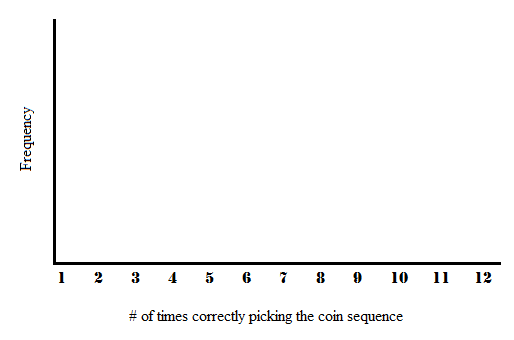
\includegraphics[width=0.5\linewidth]{../plots/Act1-NullDist.png}
\begin{students}
  \vspace{1cm}
\end{students}    
\begin{key}
   {\it Answers will vary. AWV.}
\end{key}
 

Two possible explanations for an unusual result:
  \begin{itemize}
  \item Your instructor was merely guessing which sequence was
    generated by the coin.  If this is the case, how many times would
    you expect the instructor to have been correct? 
\begin{students}
  \vspace{1cm}
\end{students}    
\begin{key}
   {\it Half the time.}
\end{key}
 
  \item Your instructor has super secret knowledge of randomness and
    could detect the fraudulent sequences.  If this is the case, how
    many times would you expect the instructor to have been correct?
    \textit{Hint: you do not need to specify a number here, just a
      direction from a particular number.} 
\begin{students}
  \vspace{1cm}
\end{students}    
\begin{key}
   {\it More than half.}
\end{key}
 
  \end{itemize}

  \item Which of these two explanations seems more plausible given the
    data?  Explain your group's choice.
\begin{students}
  \vspace{1cm}
\end{students}    
\begin{key}
   {\it Knows something?}
\end{key}
 
\item If the class was just guessing when writing down which sequence
  was the coin, your results give an example of how many sequences a
  person \textit{could} guess correctly out of
  \underline{\hspace{1cm}}.\\
 Which values are unlikely, according to the plot?
 Is the instructor's result unlikely? 
\begin{students}
  \vspace{1cm}
\end{students}    
\begin{key}
   {\it Answers will vary. Yes - instructor is unlikely.}
\end{key}

  \item What does this tell you about your instructor?  Do you think
    he/she was guessing or can detect fraud?  Explain your answer
    using the dot plot of the class results. 
\begin{students}
  \vspace{1cm}
\end{students}    
\begin{key}
   {\it Not just guessing?}
\end{key}

\textbf{Further Exploration}

  \item What could your instructor do to make you more sure they 
        can in fact detect fraud? 
\begin{students}
  \vspace{1cm}
\end{students}    
\begin{key}
   {\it Do just as well with more such sequences.}
\end{key}

  \item If an instructor had correctly identified the coin sequence
    for 20 of 24 groups and a different instructor had correctly
    identified 10 of 12 groups, which instructor would you think is
    better at detecting fraud?  Or would they be equally effective?
    Explain.  
\begin{students}
  \vspace{1cm}
\end{students}    
\begin{key}
   {\it 20 of 24 is stronger evidence than 10 of 12.}
\end{key}
\end{enumerate}

\begin{center}
  {\bf Take Home Messages}
\end{center}
  \begin{itemize}
  \item In this course we will learn how to evaluate a claim by
    comparing observed results (Instructor's guess) to a distribution.

  \item Blind guessing between two outcomes will be correct only
    about half the time. We can create data ( via computer simulation)
    to fit the assumption of blind guessing.

  \item Unusual results will make us doubt the assumptions used to
    create the distribution.  A large number correct is evidence that
    a person was not just blindly guessing.
  \end{itemize} \vspace{1in}

{\bf Assignment}\\
\begin{itemize}
\item  Trade contact info with your group members.  Decide who will
  bring a computer to the next class.
\item   Purchase a copy of the course pack.
\item   Log in to this course on D2L. Set message forwarding to an
  account you read daily.
\item View videos 1a through 1e posted on the Videos Link of D2L.
\item  Complete {\bf D2Quiz 1} on D2L.  Note: you can save a Quiz and
  work on it several times, but you may only submit it once.
\item Read the Syllabus and ``Readings 1'' on pages 1--5 and 9--12 for
  the next class. You will be quizzed over them. 
\end{itemize}




  


